%Preamble
%
\documentclass[a4paper]{report}
%
%Packages
%
\usepackage[utf8]{inputenc} 
\usepackage[french]{babel}
\usepackage[T1]{fontenc}
\usepackage{amsmath} 
\usepackage[pdftex]{graphicx} 
\usepackage{hyperref} 
\usepackage{pdfpages}
\usepackage{appendix}
\usepackage{float}
\usepackage{afterpage}
\usepackage[xindy,toc,acronym,nonumberlist,nomain]{glossaries}
\usepackage{listingsutf8}
%Document
%
\newcommand{\HRule}{\rule{\linewidth}{0.5mm}}
\begin{document}
\begin{titlepage}
\begin{center}
	\textsc{\LARGE Programmation système}\\[1.5cm]
	\textsc{\Large Projet}\\[0.5cm]
	\HRule \\[0.4cm]
	{\huge \bfseries Rapport \\[0.4cm]}
	\HRule \\[1.5cm]
	\noindent
	\begin{minipage}{0.4\textwidth}
		\emph{Étudiants : } \\ Colin \textsc{González}, \\ Benjamin \textsc{El Krieff} et \\ Élie \textsc{Canonici}
	\end{minipage}
	\vfill
	{\large 16 mai 2016}
\end{center}
\end{titlepage}
\setcounter{secnumdepth}{0}
\section{Introduction}
Le projet de programmation système que nous devions réaliser était l'implémentation d'une primitive de programmation concurrente : les \emph{channels}. Ces derniers permettent la communication entre deux processus et de les synchroniser. De plus, une telle primitive apporte en expressivité et lisibilité du code. Un des exemples de C.A.R Hoare est de formatter des code sur plaquette de 80 colonnes en 125 colonnes. Il suffit de deux processus et un channel. Le premier processus lit caractère par caractère et transmet au deuxième processus qui écrit 125 caractère lus dans le channel avant de faire un retour à la ligne. Finalement, les channels peuvent permettre de se passer des tubes UNIX dans certains cas.
\section {Les channels comme primitive de synchronisation}
Les channels sont intéressants pour synchroniser plusieurs processus, un exemple intéressant est le crible d'Eratosthène. Les channels permettent une implémentation parallèle simple à écrire, contrairement à une implémentation sans channels, souvent contre-intuitive. Le principe est d'avoir un processus qui communique des nombres par des un channel, puis d'avoir un processus qui récupère ces entier, le premier nombre qu'il reçoit est forcément premier, il l'imprime. Par la suite il transmettra au thread suivant tous les entiers non divisible par le premier entier reçu et ainsi de suite.
Nous n'observons pas de différences d'efficacité entre une implémentation sans channels et une implémentation avec channel pour les entiers en 2 et 1000, c'est à dire 0.02 secondes. Cependant entre 2 et 10 000 il y a une différence de facteur 1,76, soit 0.29 pour les channels et 0.17 pour une implémentation multithreadée classique, et un facteur 3.7 pour les entiers entre 2 et 1 million soit 878 secondes (environ 14 minutes) pour les channels et 236 secondes (environ 4 minutes) sans les channels. Ces executions on était faite avec une machine virtuelle qui tourne sous Debian 8 avec 2048 Go de RAM et deux coeurs avec 2 threads chacun à une fréquence de 2.30 GHz. Voir la figure 1.
\begin{figure}[H]
\begin{center}
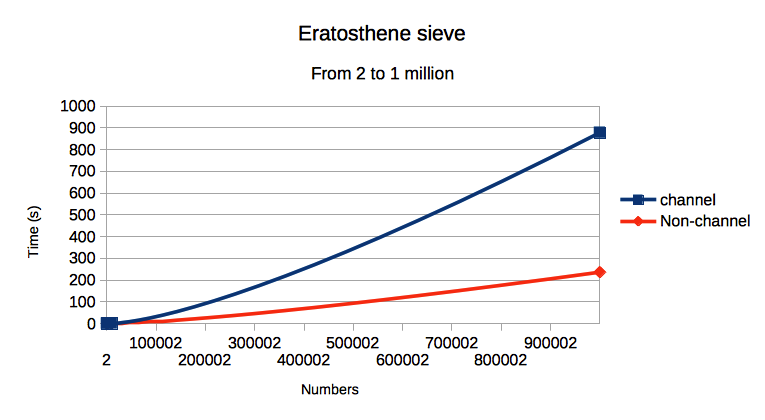
\includegraphics[width=16cm]{era-chart.png}
\caption{Crible d'Eratosthène sur une machine virtuelle Debian 8 @2.3Ghz et 2048 Mo de RAM}
\label{figure1}
\end{center}
\end{figure}

Cependant il y a un gain considérable en quand la facilité de programmation, en utilisant le logiciel sloccount l'implémentation du crible d'Eratosthène avec des channels représente 61 lignes de codes SLOC contre 93 sans les channels une économie d'un 1/3 de lignes de codes (oui, les vrais informaticiens cherchent à coder moins et plus vite, la technologie, le temps et d'autres implémentations régleront le problème de l'efficacité).
\section{Les channels à la place de tubes UNIX}
Un des TPs de cette année consistait en $n$ processus qui doivent écrire dans un même fichier. Pour éviter les conflits, ils sont organisés en anneau : le processus $pi$ est relié à $pi+1$ par un tube 1. Un jeton (entier) circule dans cet anneau, et seul le processus en possession du jeton est autorisé à accéder au fichier. Grâce aux channels \emph{globaux}, nous pouvons refaire ce programme avec des channels à la place de tubes UNIX. Pour cette exemple, nous avons fait 1000 écritures et 10 processus. L'implémentation avec channels et un peu plus rapide 4.89 secondes contre 5.10 avec les tubes UNIX, soit un écart de 0.2 secondes, en moyenne. C'est un gain de $4\%$ ce qui est négligeable. Toutefois, ce résultat est encourageant, cela signifie que l'implémentation des channels est au moins aussi efficace que les tubes UNIX.
\section{Exemples réalistes}
Les channels sont donc faciles à programmer et peuvent être efficaces selon le contexte. Pour preuve, nous avons deux programmes plausibles qui se servent des channels. Le programme fourni par le professeur, qui dessine un espace de Mandelbrot, et un un jeu de la vie. Sur l'ensemble de nos programmes nous observons que les channels synchrones sont moins rapides que les channels asynchrones, ceci dépend du nombres de threads et du nombres channels utilisés. Plus ces nombres sont importants plus le scheduler doit travailler. Par ailleurs, les channels synchrones bloquent, donc si le programme utilisateur n'est pas bien synchroniser, il peux y avoir beaucoup d'attente entre les envois et les réceptions sur les channels.
\section{Conclusion}
Grâce à ce projet de programmation nous pouvons observer que les channels ont de nombreux intérêts et nous avons appris à programmer avec les channels. De plus nous avons compris que la programmation concurrente n'apporte pas nécessairement en efficacité mais en expressivité et clarté du code. C'est exactement ce que décrivais Hoare dans les années 70 avec son langage CSP (communicating sequential processes). Le résultats expérimentaux montrent que les channels programmé en mode utilisateur peuvent être plus lents que les méthodes courantes.  Mais, ils peuvent servir efficacement comme primitive de synchronisation pour remplacer des sémaphore, des mutex et les tube UNIX. Ils facilitent la programmation de boucles à événement qui permet de se passer de threads. Par ailleurs, ils sont très facile à programmer et offrent plus d'expressivité. Ils prouvent être robustes et efficaces. Cependant, il est important des les optimiser, soit en les intégrants au langage ou au noyau pour et apprendre à les compiler efficacement.  
\end{document}
